\section{The Adding Structures}
\label{sec:add.add}

We start by plotting the periods of stable cycles in a one-dimensional scan across a period-adding structure.
\Cref{fig:minrep.adding1.motivation.halved.1d.period.full} shows this scan, while \Cref{fig:minrep.adding1.corner.period.full} shows the period-structure.
The period range on the one-dimensional scan is marked in red between the regions $P_{10}^4$ and $P_{10}^4 \oplus P_9^4$.
The regions $P_{10}^4$ and $P_9^4$ have cycles as we expect, $\Cycle{\A^6\B^4\C^6\D^4}$ and $\Cycle{\A^5\B^4\C^5\D^4}$.
But the region $P_{10}^4 \oplus P_9^4$ is weirder.
In this region, there are two coexisting cycles, that act like the coexisting cycles in ``type B'' parameter regions.
They are hybrids of the cycles $P_{10}^4$ and $P_9^4$, $\Cycle{\A^6\B^4\C^5\D^4}$ and $\Cycle{\A^5\B^4\C^6\D^4}$, acting like one cycle on the one half of the model and acting like the other cycles on the other half.
This is the first sign, that there is something off about this period-adding structure.

Examining the one-dimensional scan of the period-adding structure, \Cref{fig:minrep.adding1.motivation.halved.1d.period.full}, closer we find some inconsistencies.
First, the period of the cycle $\sigma\rho$, 58, is larger than the periods of $\sigma$, 20, and $\rho$, 19, combined.
This is unexpected because the cycle $\sigma\rho$ should be the cycles $\sigma$ and $\rho$ glued together, and therefore its period should be exactly the sum of the periods of the cycles $\sigma$ and $\rho$.
Similarly, the period of $\sigma^2\rho$ should be the sum of the periods of $\sigma$ and $\sigma\rho$.
But instead, the period of $\sigma^2\rho$ is smaller than the period of $\sigma\rho$.
Is this not a period-adding cascade after all?

What is happening here is that a period-adding structure in the halved model manifests as this weird structure in the full model.
This becomes apparent when simulating the halved model in the same period ranges.
\Cref{fig:minrep.adding1.motivation.halved.1d.period.halved} shows the one-dimensional period scan in the halved model that corresponds to the scan in the full model in \Cref{fig:minrep.adding1.motivation.halved.1d.period.full}.
In the halved model, $\sigma$ is the cycle $\Cycle{\L^6\R^4}$, which is expected for the cycle $P_{10}^4$, and $\rho$ is the cycle $\Cycle{\L^6\R^4\L^5\R^4}$.
The cycle $\sigma\rho$ in between the two is now actually the two cycles glued together $\Cycle{(\L^6\R^4)^2\L^5R^4}$, as we would expect in a period-adding structure.
And its period is 29, which is the sum of the periods of the cycle $\sigma$, 10, and $\rho$, 19.

Now we can also see that the unusual hybrid cycles $P_{10}^4 \oplus P_9^4$ in the full model are the manifestation of the cycle $\Cycle{L^6\R^4\L^5\R^4}$ in the halved model.
This cycle is itself the first level of the real period-adding structure of the cycles $P_{10}^4$ and $P_9^4$, which are $\Cycle{\L^6\R^4}$ and $\Cycle{L^5\R^4}$ in the halved model.
\Cref{fig:minrep.adding1.large.adding} shows a one-dimensional scan of a full period-adding structure in the halved model at different parameter values that allow for larger period regions with higher periods, making them visible to us.
In the next section, we will explain what exactly the halved model is, why it works in our case, and how to translate symbolic sequences between it and the full model.

\begin{figure}
	\centering
	\subfloat[The full model]{
		\includegraphics[width=.4 \textwidth]{62_MinimalRepr_Adding/2D_Period_1_Zoomed/result.png}
		\label{fig:minrep.adding1.corner.period.full}
	}
	\subfloat[The halved model]{
		\includegraphics[width=.4 \textwidth]{63_MinimalRepr_Adding_Halved/2D_Period_1_Zoomed/result.png}
		\label{fig:minrep.adding1.corner.period.halved}
	}
	\caption{
		2D period scans of period-adding regions of the same model in two different versions.
		On the left, is the full version of the model and on the right, is the halved version of the model.
		The red markers between the regions $P_{10}^4$ and $P_{10}^4 \oplus P_9^4$ in both pictures, is the parameter range used for the 1D scans in \Cref{fig:minrep.adding1.motivation.halved.1d.period}.
	}
	\label{fig:minrep.adding1.corner.period}
\end{figure}

\begin{figure}
	\centering
	\subfloat[The full model]{
		\includegraphics[width=.4 \textwidth]{62_MinimalRepr_Adding/1D_Period_1_add_hor_D1/result.png}
		\label{fig:minrep.adding1.motivation.halved.1d.period.full}
	}
	\subfloat[The halved model]{
		\includegraphics[width=.4 \textwidth]{63_MinimalRepr_Adding_Halved/1D_Period_1_add_hor_D1/result.png}
		\label{fig:minrep.adding1.motivation.halved.1d.period.halved}
	}
	\caption{
		1D period scans of a period-adding cascade of the same model in two different versions.
		On the left, is the full version of the model and on the right, is the halved version of the model.
		The parameter range is the same in both models and is marked red in \Cref{fig:minrep.adding1.corner.period}.
	}
	\label{fig:minrep.adding1.motivation.halved.1d.period}
\end{figure}

\begin{figure}
	\centering
	\includegraphics[width=.7 \textwidth]{63_MinimalRepr_Adding_Halved/1D_Period_larger_adding/result.png}
	\caption{
		A 1D period scan of a horizontal adding structure at parameter values that allow us to see the adding more clearly.
		The fixed parameter values are $a_L = 1, b_L = 0.8, p_x = -0.39$ and $p_y$ is in the range $[0.082, 0.087]$.
		The cycles involved in the adding are $P_7^3$ and $P_7^2$.
	}
	\label{fig:minrep.adding1.large.adding}
\end{figure}

\begin{figure}
	\centering
	\includegraphics[width=\textwidth]{FareyTrees/Minrep_Adding1_Halved/adding.png}
	\caption{t}
	\label{fig:tree.adding1.hor.halved}
\end{figure}

\begin{figure}
	\centering
	\includegraphics[width=\textwidth]{FareyTrees/Minrep_Adding1_Full/adding.png}
	\caption{t}
	\label{fig:tree.adding1.hor.full}
\end{figure}

\subsection{The Halved Model}

The idea behind the halved model is that the model we have can be looked at in a different way than it was introduced in.
We know the model $m$ maps an input $x$ to $f(x) \mod 1$, meaning that if the output $f(x)$ is greater or equal to 1, we subtract 1 from it until it is in the range $[0, 1)$.
Similarly, we add 1 to it if it is smaller than 0 until it is in the desired range.
Now instead of confining the model to the domain of $[0, 1)$, we think of it repeating infinitely in both directions.
This proces is called lifting of circle maps and is described by \Citeauthor{devaney2021introduction} in his book~\cite{devaney2021introduction}.
We can achieve this by mapping $T^m: x \mapsto f(x - \lfloor x \rfloor)$.
This trick maps the input $x$ into the domain, on which our model function produces sensible results and causes it to repeat infinitely.
$T^m$ is now a lift of the model $m$ in the domain of all real numbers $\mathbb{R}$.
\Cref{fig:minrep.infinite.model.concept} illustrates this concept for the cycle $P_7^3$.
The blue square is the full model.
One can see, that the branch $f_\D$ is outside the blue square at its right edge.
This is because it was cut off and continued at the bottom of the square before, due to the $\mod 1$ operation.

\todo{this makes sense in the original problem domain}

In this model, there are no cycles that have multiple rotations.
Instead, the cycles that had multiple rotations in the full model, manifest as a sequence of different blocks of the full model.
Meaning for the example $P_7^3$, the same blocks of $\A^4\B^3\C^4\D^3$ are repeating infinitely.
But for an example with multiple rotations, such as $\A\B\C\D\A^2\B^2\C^2\D^2$, the blocks will not all be the same.
Instead, the blocks $\A\B\C\D$ and $\A^2\B^2\C^2\D^2$ will be alternating.

Now the symmetry of our function $f$ comes into play.
Since $f(x + 0.5) = f(x) + 0.5$ for $x \in [0, 0.5)$, we can split the infinite model into smaller blocks than the blue block of the full model.
The function of the infinite model repeats in blocks of size 0.5, these blocks are marked red in \Cref{fig:minrep.infinite.model.concept}.
These red blocks represent the halved model, it is the smallest repeating part of the infinite model $T^m$.
Basically we choose the smallest model, of which $T^m$ is a lift.
This happens to be exactly our model $m$ folded in half.
Se the halved model $h$ is defined on the interval $[0, \frac{1}{2})$ and maps $x \mapsto g(x) \mod \frac{1}{2}$, where $g(x)$ is the same as in our model $m$, defined in \Cref{sec:minrep.definition}.

To get the symbolic sequence of a cycle in the halved model, we look at the pattern in which different red blocks repeat along the infinite model.
For our example in the picture, there is only one red block that repeats infinitely, $\L^4\R^3$.
The next section will explain, how to translate cycles between the halved and full model.

\begin{figure}
	\centering
	\includegraphics[width=.7 \textwidth]{63_MinimalRepr_Adding_Halved/Cob_Vis_s/Manual/result.png}
	\caption{Illustration of the infinite model concept.}
	\label{fig:minrep.infinite.model.concept}
\end{figure}

\subsection{Translating Symbolic Sequences}

\todo{intro paragraph}

\todo{mention that $\sigma, \rho, \tau$ are symb seq in the halved model, $\phi, \psi, \pi$ in the full model}

\subsubsection{Naive Algorithm}

Based on this concept of the infinite model, one can formulate a naive algorithm for translating symbolic sequences between the halved and full model.
We will start with the easier direction from the full to the halved model.
From this direction we can't learn much about the nature of the period-adding structure in the full model, the inverse will be more important for that.

To translate a symbolic sequence of the full model we start by writing it down.
For example $\phi = \A^4\B^3\C^4\D^3$.
Then we replace the symbols $\A$ and $\C$ by $\L$ and the symbols $\B$ and $\D$ by $\R$.
Now we have $\L^4\R^3\L^4\R^3$.
Finally, we have to check for redundancy in the resulting cycle.
In our example, the cycle $\L^4\R^3$ repeats twice in $\L^4\R^3\L^4\R^3$, so we just keep $\L^4\R^3$.

The inverse is trickier.
We start by writing down the symbolic sequence in the halved model.
For example $\sigma = \L^4\R^3\L4\R^3\L^3\R^3$.
Now we need to build pairs of rotations since each blue block fits two red blocks.
If there is one rotation left over at the end, we wrap around or equivalently write down the original sequence again.
We repeat this until we fit all rotations that we have written down.

\begin{lemma}[How Often Do We Have To Write Down the Symbolic Sequence]
	\label{lemma:writing.down}
	For cycles in the halved model $\sigma$ with an even number of rotations $n$, we only need to write the original cycle down once.
	For cycles in the halved model $\sigma$ with an odd number of rotations $n$, we need to write the original cycle down exactly twice.
\end{lemma}

\begin{proof} \phantom{x}
	\begin{enumerate}
		\item Let $n = 2i$. Then, we can build $i$ pairs of rotations and fit all $2i$ rotations of the original model.
		\item Let $n = 2i + 1$. We start by building $i$ pairs of rotations, fitting $2i$ rotations.
		      This will leave the last rotation unpaired, so we write down the sequence of $2i + 1$ rotations again.
		      Now we can pair up the last rotation of the first sequence we wrote down with the first rotation of the sequence we just wrote down.
		      $2i$ rotations remain, which we can fit into $i$ pairs.
	\end{enumerate}
\end{proof}

Notice, our example symbolic sequence has 3 rotations.
This means we have to write down the original sequence twice $\sigma^2 = \L^4\R^3\L4\R^3\L^3\R^3\L^4\R^3\L4\R^3\L^3\R^3$.

Then we pair up the rotations, this corresponds to drawing blue boxes around the red boxes in the infinite model.
In our example, we get the pairs $(\L^4\R^3\L^4\R^3)(\L^3\R^3\L^4\R^3)(\L^4\R^3\L^3\R^3)$.
The pairs then have to be translated using the function $t$ defined below in \Cref{def:t}.
The resulting symbolic sequence is $T(h) = \A^4\B^3\C^4\D^3\A^3\B^3\C^4\D^3\A^4\B^3\C^3\D^3$.
The formal definition of $T$ is below in \Cref{def:T}.

\begin{definition}[Syllables]
	A syllable is a sequence of the same symbol if it can't be extended in the context of the symbolic sequence it is in.
	So for example, $\L^3$ is a syllable in $\L^3\R^3$, but $\L^2$ and $\L$ are not.
	A 2-syllable is a pair of syllables that are next to each other.
	And a 4-syllable is a pair of 2-syllables that are next to each other.

	In the halved model, a 2-syllable corresponds to one rotation.
	In the full model, a 4-syllable corresponds to one rotation.
	These terms are used interchangably in the rest of this chapter.
\end{definition}

\begin{definition}[Translation of 4-syllables from the Halved Model to the Full Model $t$]
	\label{def:t}
	The function $t$ maps two rotations, or a 4-syllable, of a symbolic sequence in the halved model to a single rotation in the full model.
	It is defined in the following way.
	\begin{align}
		t: & \L^a\R^b\L^c\R^d \mapsto \A^a\B^b\C^c\D^d
	\end{align}
\end{definition}

\begin{definition}[Translation of a Symbolic Sequence from the Halved Model to the Full Model $T$]
	\label{def:T}
	The function $T$ translates a symbolic sequence $\sigma = \sigma_1\sigma_2 \dots \sigma_n$ in the halved model to the full model.
	Where $\sigma_i$ are the 2-syllables of $\sigma$.
	From \Cref{lemma:writing.down} we know how often we need to write down $\sigma$, and therefore also which 4-syllables to translate with $t$.
	\begin{align}
		T(\sigma) & = \begin{cases}
			              t(\sigma_1\sigma_2) \dots t(\sigma_{n-1}\sigma_n)                           & \text{ if } n | 2 \\
			              t(\sigma_1\sigma_2) \dots t(\sigma_n\sigma_1) \dots t(\sigma_{n-1}\sigma_n) & \text{ else }
		              \end{cases}
	\end{align}
\end{definition}

\begin{definition}[Shifting Symbolic Sequences]
	The function $s_2$ shifts a symbolic sequence $\sigma$ in the halved model by a single rotation, or equivalently by a 2-syllable.
	Let $\sigma = \sigma_1\sigma_2 \dots \sigma_n$, where $\sigma_i$ are 2-syllables.
	Then $s_2$ is defined in the following way.
	\begin{align}
		s: & \sigma_1\sigma_2 \dots \sigma_n \mapsto \sigma_2 \dots \sigma_n\sigma_1
	\end{align}
	In the full model, there is a similar function, $s_4$, that shifts a symbolic sequence $\phi$ in the full model by a single rotation.
	Let $\phi = \phi_1\phi_2 \dots \phi_n$, where $\phi_i$ are 4-syllables.
	Then $s_4$ is defined in the following way.
	\begin{align}
		s_4: & \phi_1\phi_2 \dots \phi_n \mapsto \phi_2 \dots \phi_n\phi_1
	\end{align}
\end{definition}

\begin{definition}[Shift-equivalence]
	The two symbolic sequences $\phi$ and $\psi$ in the full model are shift-equivalent $\phi \equiv \psi$,
	if they both have the same number of rotations $n$
	and there is a number $0 \leq i < n$, such that $\phi = s_4^i(\psi)$.
	Where $s_4^i$ is the same as applying $s_4$ $i$ times.
	\todo{better proof, inductive}
\end{definition}

We need to repeat the whole process for each shift $s_2^i$ of the original symbolic sequence for $0 < i < n$ where $n$ is the number of rotations, or equivalently 2-syllables, of the original symbolic sequence.
And we only keep the results that are not shift-equivalent to any previous result.
In our example, we would repeat the process for $s_2(\sigma) = \L^4\R^3\L3\R^3\L^4\R^3$ and get the result $T(s_2(\sigma)) = \A^4\B^3\C^3\D^3\A^4\B^3\C^4\D^3\A^3\B^3\C^4\D^3$.
This result is shift-equivalent to the first result by shifting it 2 times ($s_4^2$).
Last we need to repeat it for $s_2^2(\sigma) = \L^3\R^3\L4\R^3\L^4\R^3$ and get the result $T(s_2^2(\sigma)) = \A^3\B^3\C^4\D^3\A^4\B^3\C^3\D^3\A^4\B^3\C^4\D^3$.
This result is shift-equivalent to the first result by shifting it once ($s_4$).

Therefore the cycle $\sigma$ in the halved model manifests as a single cycle $T(\sigma)$ in the full model.
We write it as $F(\sigma) = \{T(\sigma)\} = \{\A^4\B^3\C^4\D^3\A^3\B^3\C^4\D^3\A^4\B^3\C^3\D^3\}$.
The result of $F$ is a set because the cycle $\sigma$ in the halved model may manifest as multiple coexisting cycles in the full model.

\subsubsection{Properties of Translated Symbolic Sequences in the Full Model}

With this naive algorithm, we can start to investigate rules for the period-adding structure in the full model.

\begin{lemma}[Shif-equivalence of Translated Symbolic Sequences]
	\label{lemma:equivalence.translations}
	The translations of the two cycles $\sigma$ and $\rho = s_2^{2i}(\sigma)$ in the halved model are shift-equivalent $T(\sigma) \equiv T(\rho)$ in the full model for all integers $i$.
\end{lemma}

\begin{proof}
	Let $\sigma = \sigma_1\sigma_2 \dots \sigma_n$, therefore $\rho = \sigma_{2i+1} \dots \sigma_n\sigma_1 \dots \sigma_{2i}$.
	The translations are $T(\sigma) = t(\sigma_1\sigma_2)t(\sigma_3\sigma_4) \dots t(\sigma_{n-1}\sigma_n)$
	and $T(\rho) = t(\sigma_{2i+1}\sigma_{2i+2}) \dots t(\sigma_{n-1}\sigma_n)t(\sigma_1\sigma_2) \dots t(\sigma_{2i-i}\sigma_{2i})$.
	We can see that $T(\rho) = s_4^i(T(\sigma))$ and therefore $T(\sigma) \equiv T(\rho)$.
\end{proof}

\begin{theorem}[Coexistence of Translated Symbolic Sequences]
	\label{theorem:coexistence.even}
	The mainfestations of a cycle in the halfed model $\sigma$ is either $F(\sigma) = \{T(\sigma), T(s_2(\sigma))\}$ or $F(\sigma) = \{T(\sigma)\}$.
	And \begin{enumerate}
		\item $F(\sigma) = \{T(\sigma), T(s_2(\sigma))\}$ if the number of rotations of the sequence $\sigma$ is even.
		\item $F(\sigma) = \{T(\sigma)\}$ if the number of rotations of the sequence $\sigma$ is odd.
	\end{enumerate}
\end{theorem}

\begin{proof}
	Let $\sigma = \sigma_1\sigma_2 \dots \sigma_n$ a symbolic sequence in the halved model with $n$ rotations.
	We know from \Cref{lemma:equivalence.translations} that the only possible candidates for $F(\sigma)$ are $T(\sigma)$ and $T(s_2(\sigma))$.
	These are the first two possibilities we check in the algorithm and all other shifts $T(s_2^i(\sigma))$ with $2 \leq i < n$ are shift-equivalent to $T(\sigma)$ or $T(s_2(\sigma))$.
	This follows directly from \Cref{lemma:equivalence.translations}.
	So, in the following, we will only check for the shift-equivalence of these two candidates.
	\begin{enumerate}
		\item Let $n = 2i$.
		      \begin{align*}
			              & T(h) = t(\sigma_1\sigma_2) t(\sigma_3\sigma_4) \dots t(\sigma_{n-1}\sigma_n)  \\
			      \nequiv & T(s_2(h)) = t(\sigma_2\sigma_3) t(\sigma_4\sigma_5) \dots t(\sigma_n\sigma_1)
		      \end{align*}
		      The two candidates are not shift-equivalent because the pair $t(\sigma_1\sigma_2)$ in $T(\sigma)$ is not included in the other candidate $T(s_2(\sigma))$.
		      The same is true for any other pair, and therefore $F(\sigma) = \{T(\sigma), T(s_2(\sigma))\}$.
		\item Let $n = 2i + 1$.
		      \begin{align*}
			             & T(h) = t(\sigma_1\sigma_2) t(\sigma_3\sigma_4) \dots t(\sigma_n\sigma_1) t(\sigma_2\sigma_3) \dots t(\sigma_{n-1}\sigma_n)      \\
			      \equiv & T(s_2(h)) = t(\sigma_2\sigma_3) \dots t(\sigma_{n-1}\sigma_n) t(\sigma_1\sigma_2) t(\sigma_3\sigma_4) \dots t(\sigma_n\sigma_1)
		      \end{align*}
		      The two candidates are shift-equivalent.
		      By shifting the second candidate $T(s_2(\sigma))$ $2i$ times, we get the first candidate $T(\sigma)$.
		      Therefore, the second candidate is discarded and $F(\sigma) = \{T(\sigma)\}$.
	\end{enumerate}
\end{proof}

Note that a result of $F(\sigma) = \{T(\sigma), T(s_2(\sigma))\}$ means that the cycle in the halved model $\sigma$ manifests as two coexisting cycles in the full model.

\subsubsection{Revised Algorithm}

With all these properties and functions we now can formulate a more compact algorithm, \Cref{alg:halved.to.full}, for translating symbolic sequences from the halved model into the full model.
This revised algorithm will be used in the following to explain the rules of the period-adding structure in the full model.

\begin{algorithm}
	\caption{Translating a Symbolic Sequence from the Halved Model to the Full Model}\label{alg:halved.to.full}
	\begin{algorithmic}
		\Require $\sigma = \sigma_1\sigma_2 \dots \sigma_n$ with $n > 0$
		\If{$n$ is even}
		\State \Return $\{t(\sigma_1\sigma_2) t(\sigma_3\sigma_4) \dots t(\sigma_{n-1}\sigma_n), t(\sigma_2\sigma_3) t(\sigma_4\sigma_5) \dots t(\sigma_n\sigma_1)\}$
		\ElsIf{$n$ is odd}
		\State \Return $\{t(\sigma_1\sigma_2) \dots t(\sigma_{n}\sigma_1) \dots t(\sigma_{n-1}\sigma_n)\}$
		\EndIf
	\end{algorithmic}
\end{algorithm}

\Cref{alg:full.to.halved} shows the inverse algorithm for translating symbolic sequences from the full model to the halved model for completeness.
It uses the inverse $t^{-1}$ of the function $t$.

\begin{definition}[The inverse of $t$]
	The function $t^{-1}$ maps one rotation of a symbolic sequence in the full model to two rotations in the halved model.
	It is defined in the following way.
	\begin{align}
		t^{-1}: & \A^a\B^b\C^c\D^d \mapsto \L^a\R^b\L^c\R^d
	\end{align}
\end{definition}

\begin{algorithm}
	\caption{Translating a Symbolic Sequence from the Full Model to the Halved Model}\label{alg:full.to.halved}
	\begin{algorithmic}
		\Require $\phi = \phi_1\phi_2 \dots \phi_n$ with $n > 0$
		\State $d \gets t^{-1}(\phi_1)t^{-1}(\phi_2) \dots t^{-1}(\phi_n) = \sigma_1\sigma_2 \dots \sigma_m$
		\Comment $m = 2n$ is even
		\State $\tau \gets \sigma_1\sigma_2 \dots \sigma_{\frac{m}{2}}$
		\If{$\sigma = \tau^2$}
		\State \Return $\tau$
		\ElsIf{$\sigma \neq \tau^2$}
		\State \Return $\sigma$
		\EndIf
	\end{algorithmic}
\end{algorithm}

\subsection{Properties of the Period-adding Structure in the Full Model}

With this knowledge, we now can explain, why some cycles in the full model have a much lower period than expected in period-adding structures.

\begin{lemma}[$t$ Preserves Period]
	\label{lemma:t.preserves.period}
	The function $t$ preserves the period. $|\sigma_1\sigma_2| = |t(\sigma_1\sigma_2)|$.
\end{lemma}

\begin{proof}
	Let $\sigma_1\sigma_2 = \L^a\R^b\L^c\R^d$.
	\begin{align*}
		|\sigma_1\sigma_2| =  |\L^a\R^b\L^c\R^d|
		= a + b + c + d
		= |\A^a\B^b\C^c\D^d|
		= |t(\L^a\R^b\L^c\R^d)|
		= |t(\sigma_1\sigma_2)|
	\end{align*}
\end{proof}

\begin{theorem}[Period of Cycles in the Full Model]
	\begin{enumerate}
		\item If a cycle in the halved model manifests as two coexisting cycles in the full model, the period of either cycle is the same as the period of the cycle in the halved model. $|T(\sigma)| = |T(s_2(\sigma))| = |\sigma|$.
		\item If a cycle in the halved model manifests as a single cycle in the full model, the period of this cycle is double the period of the cycle in the halved model. $|T(\sigma)| = 2 |\sigma|$.
	\end{enumerate}
\end{theorem}

\begin{proof} \phantom{x}
	\begin{enumerate}
		\item From \Cref{theorem:coexistence.even} we know that if the cycle $\sigma$ in the halved model manifests as two coexisting cycles in the full model, $\sigma$ has an even number of rotations $n$.
		      And its translation is $T(\sigma) = t(\sigma_1\sigma_2) t(\sigma_3\sigma_4) \dots t(\sigma_{n-1}\sigma_n)$.
		      Combining this with the fact, that $t$ preserves the period of its input as described in \Cref{lemma:t.preserves.period}, we can calculate the period of $T(h)$ in the following way.
		      \begin{align*}
			      |T(h)| & = |t(\sigma_1\sigma_2) t(\sigma_3\sigma_4) \dots t(\sigma_{n-1}\sigma_n)|           \\
			             & = |t(\sigma_1\sigma_2)| + |t(\sigma_3\sigma_4)| + \dots + |t(\sigma_{n-1}\sigma_n)| \\
			             & = |\sigma_1\sigma_2| + |\sigma_3\sigma_4| + \dots + |\sigma_{n-1}\sigma_n|          \\
			             & = |\sigma_1\sigma_2 \dots \sigma_n| = |h|
		      \end{align*}
		      So the period of the cycle $T(\sigma)$ in the full model is the same as the period of the cycle $\sigma$ in the halved model.
		      The same calculation can be done for $T(s(\sigma))$ and is omitted here.
		\item Similarly we know that if the cycle $\sigma$ in the halved model manifests as a single cycle in the full model, $\sigma$ has an odd number of rotations $n$.
		      And its translation is $T(\sigma) = t(\sigma_1\sigma_2) \dots t(\sigma_n\sigma_1) \dots t(\sigma_{n-1}\sigma_n)$.
		      Its period can be calculated in the following way.
		      \begin{align*}
			      |T(h)| & = |t(\sigma_1\sigma_2) \dots t(\sigma_n\sigma_1) \dots t(\sigma_{n-1}\sigma_n)|                      \\
			             & = |t(\sigma_1\sigma_2)| + \dots + |t(\sigma_n\sigma_1)| + \dots + |t(\sigma_{n-1}\sigma_n)|          \\
			             & = |\sigma_1\sigma_2| + \dots + |\sigma_n\sigma_1| + \dots + |\sigma_{n-1}\sigma_n|                   \\
			             & = |\sigma_1\sigma_2 \dots \sigma_n\sigma_1 \dots \sigma_{n-1}\sigma_n| = |\sigma\sigma| = 2 |\sigma|
		      \end{align*}
		      So the period of the cycle $T(\sigma)$ in the full model is twice the period of the cycle $\sigma$ in the halved model.
	\end{enumerate}
\end{proof}

\subsubsection{Rules for Combining Symbolic Sequences}

Looking at the farey tree in \Cref{fig:tree.adding1.hor.full}, we can see some regularities in the distribution of coexisting (yellow) and single (white) cycles in the full model.
These can be explained with \Cref{theorem:coexistence.even}.
\todo{last case not possible in our adding structures. proof!}
The third case in \Cref{theorem:child.coexistence} can't be seen in the farey tree but it follows from the proof of the first two cases.

\begin{theorem}[Multiplicity of Cycles Associated With Child Nodes Based on the Multiplicity of Cycles Associated With its Parent Nodes]
	\label{theorem:child.coexistence}
	\begin{enumerate}
		\item The child of a node with a single cycle and a node with two coexisting cycles has a single cycle.
		\item The child of two nodes with a single cycle has two coexisting cycles.
		\item The child of two nodes with two coexisting cycles, has two coexisting cycles.
	\end{enumerate}
\end{theorem}

\begin{proof} \phantom{x}
	\begin{enumerate}
		\item A node with a single cycle in the full model is the manifestation of a cycle with an odd number of rotations in the halved model.
		      A node with two coexisting cycles in the full model is the manifestation of a cycle with an even number of rotations in the halved model.
		      Their child is the manifestation of the two cycles in the halved model glued together.
		      This glued-together cycle has an odd number of rotations and therefore manifests as a single cycle in the full model.
		\item Analogously, two cycles with an odd number of rotations glued together have an even number of rotations.
		      Therefore, this glued-together cycle manifests as two coexisting cycles in the full model.
		\item Analogously, two cycles with an even number of rotations glued together have an even number of rotations.
		      Therefore this glued-together cycle manifests as two coexisting cycles in the full model.
	\end{enumerate}
\end{proof}

Furthermore, we can formulate rules for the cycles in the child node of two nodes in the period-adding structure in the full model.

\begin{definition}[Merging two 4-syllables]
	The operation $\left[\phi_i \mid \psi_j\right]$ merges the two 4-symmables $\phi_i$ and $\psi_j$.
	Let $\phi_i = \A^a\B^b\C^c\D^d$ and $\psi_j = \A^e\B^f\C^g\D^h$.
	Then $\left[\phi_i \mid \psi_j\right] = \A^a\B^b\C^g\D^h$.
	It concatenates the first 2-syllable of $\phi_i$ with the second 2-syllable of $\psi_j$.
\end{definition}

\begin{theorem}[The Cycles of a Child Node of a Node With a Singular Cycle and a Node With 2 Coexisting Cycles]
	The child node of a node with a singular cycle $\phi = \phi_1\phi_2 \dots \phi_n$ and a node with two coexisting cycles $\phi^a = \phi^a_1\phi^a_2 \dots \phi^a_m$ and $\phi^b_1\phi^b_2 \dots \phi^b_m$ will have one of the following cycles.
	\begin{enumerate}
		\item If $\phi$ is associated with the left parent.
		      \begin{align*}
			      \phi_1 \dots \phi_{\frac{n-1}{2}} \left[\phi_{\frac{n+1}{2}} \mid \phi^b_m\right]
			      \phi^b_1 \dots \phi^b_{m-1} \left[\phi^b_m \mid \phi_{\frac{n+1}{2}}\right]
			      \phi_{\frac{n+3}{2}} \dots \phi_n \phi^a
		      \end{align*}
		\item If $\phi$ is associated with the right parent.
		      \begin{align*}
			      \phi^a \phi_1 \dots \phi_{\frac{n-1}{2}} \left[\phi_{\frac{n+1}{2}} \mid \phi^b_m\right]
			      \phi^b_1 \dots \phi^b_{m-1} \left[\phi^b_m \mid \phi_{\frac{n+1}{2}}\right]
			      \phi_{\frac{n+3}{2}} \dots \phi_n
		      \end{align*}
		      Which is shift-equivalent to the first case.
		      But this distinction must be made to guarantee the correctness of cycles in subsequent child nodes.
	\end{enumerate}
\end{theorem}

\begin{proof} \phantom{x}
	\begin{enumerate}
		\item Let $\sigma = \sigma_1\sigma_2 \dots \sigma_i$ with odd $i$ and $\rho = \rho_1\rho_2 \dots \rho_j$ with even $j$ and $T(\sigma) = \phi, T(\rho) = \psi^a$, and $T(s_2(\rho)) = \psi^b$.
		      The child of both nodes in the halved model will have the cycle $\sigma\rho = \sigma_1\sigma_2 \dots \sigma_i \rho_1\rho_2 \dots \rho_j$.
		      This will manifest as the following cycle in the full model.
		      \begin{align*}
			      T(\sigma\rho) & = T(\sigma_1 \dots \sigma_i \rho_1 \dots \rho_j)                                                                              \\
			                    & =
			      t(\sigma_1\sigma_2) \dots t(\sigma_i \rho_1) \dots t(\rho_j \sigma_1) \dots t(\sigma_{i-1}\sigma_i) t(\rho_1\rho_2) \dots t(\rho_{j-1}\rho_j) \\
			                    & = \phi_1 \dots \phi_{\frac{n-1}{2}} t(\sigma_i \rho_1)
			      \psi^b_1 \dots \rho^b_{m-1} t(\rho_j \sigma_1)
			      \phi_{\frac{n+3}{2}} \dots \phi_n
			      \psi^a_1 \dots \psi^a_m                                                                                                                       \\
			                    & =
			      \phi_1 \dots \sigma_{\frac{n-1}{2}} \left[\sigma_{\frac{n+1}{2}} \mid \rho^b_m\right]
			      \psi^b_1 \dots \psi^b_{m-1} \left[\rho^b_m \mid \sigma_{\frac{n+1}{2}}\right]
			      \phi_{\frac{n+3}{2}} \dots \phi_n
			      \psi^a                                                                                                                                        \\
		      \end{align*}
		\item Let $\sigma = \sigma_1\sigma_2 \dots \sigma_i$ with even $i$ and $\rho = \rho_1\rho_2 \dots \rho_j$ with odd $j$ and $T(\sigma) = \psi^a, T(s_2(\sigma)) = \psi^b$, and $T(\rho) = \phi$.
		      The child of both nodes in the halved model will have the cycle $\sigma\rho = \sigma_1l_2 \dots \sigma_i \rho_1\rho_2 \dots \rho_j$.
		      This will manifest as the following cycle in the full model.
		      \begin{align*}
			      T(\sigma\rho) & = T(\sigma_1 \dots \sigma_i \rho_1 \dots \rho_j)                                                                                             \\
			                    & =
			      t(\sigma_1\sigma_2) \dots t(\sigma_{i-1}\sigma_i) t(\rho_1\rho_2) \dots t(\rho_j \sigma_1) \dots t(\sigma_i\rho_1) \dots t(\rho_j\sigma_1) \dots t(\sigma_i) \\
			                    & =
			      \psi^a_1 \dots \psi^a_m
			      \phi_1 \dots \phi_{\frac{n-1}{2}} t(\sigma_i \rho_1)
			      \psi^b_1 \dots \psi^b_{m-1} t(\rho_j \sigma_1)
			      \phi_{\frac{n+3}{2}} \dots \phi_n                                                                                                                            \\
			                    & =
			      \psi^a
			      \phi_1 \dots \phi_{\frac{n-1}{2}} \left[\phi_{\frac{n+1}{2}} \mid \psi^b_m\right]
			      \psi^b_1 \dots \psi^b_{m-1} \left[\psi^b_m \mid \phi_{\frac{n+1}{2}}\right]
			      \phi_{\frac{n+3}{2}} \dots \phi_n                                                                                                                            \\
		      \end{align*}
	\end{enumerate}
\end{proof}

\begin{theorem}
	The child node of two nodes with a singular cycle, $\phi = \phi_1 \dots \phi_n$ and $\psi = \psi_1 \dots \psi_m$ respectively, has the following two cycles.
	\begin{align*}
		\phi_1 \dots \phi_{\frac{n-1}{2}} \left[\phi_{\frac{n+1}{2}} \mid \psi_{\frac{m+1}{2}}\right] \psi_{\frac{m+3}{2}} \dots \psi_m
	\end{align*}
	and
	\begin{align*}
		\phi_{\frac{n+3}{2}} \dots \phi_n \psi_1 \dots \psi_{\frac{m-1}{2}} \left[\psi_{\frac{m+1}{2}} \mid \phi_{\frac{n+1}{2}}\right]
	\end{align*}
\end{theorem}

\begin{proof}
	Let $\sigma = \sigma_1\sigma_2 \dots \sigma_i$ with odd $i$ and $\rho = \rho_1\rho_2 \dots \rho_j$ with odd $j$ and $T(\sigma) = \phi$ and $T(\rho) = \psi$.
	The child of both nodes in the halved model will have the cycle $\sigma\rho = \sigma_1 \dots \sigma_i \rho_1 \dots \rho_j$.
	This will manifest as the following two cycles in the full model.
	\begin{align*}
		T(\sigma\rho) & = T(\sigma_1 \dots \sigma_i \rho_1 \dots \rho_j)                                                                                  \\
		              & = t(\sigma_1\sigma_2) \dots t(\sigma_i\rho_1) \dots t(\rho_{j-1}\rho_j)                                                           \\
		              & = \phi_1 \dots \phi_{\frac{n-1}{2}} t(\sigma_i\rho_1) \psi_{\frac{m+3}{2}} \dots \psi_j                                           \\
		              & = \phi_1 \dots \phi_{\frac{n-1}{2}} \left[\phi_{\frac{n+1}{2}} \mid \psi_{\frac{m+1}{2}}\right] \psi_{\frac{m+3}{2}} \dots \psi_j
	\end{align*}
	and
	\begin{align*}
		T(s(\sigma\rho)) & = T(\sigma_2 \dots \sigma_i \rho_1 \dots \rho_j \sigma_1)                                                                         \\
		                 & = t(\sigma_2\sigma_3) \dots t(\sigma_{i-1}\sigma_i) t(\rho_1\rho_2) \dots t(\rho_j\sigma_1)                                       \\
		                 & = \phi_{\frac{n+3}{2}} \dots \phi_n \psi_1 \dots \psi_{\frac{m-1}{2}} t(\rho_j\sigma_1)                                           \\
		                 & = \phi_{\frac{n+3}{2}} \dots \phi_n \psi_1 \dots \psi_{\frac{m-1}{2}} \left[\psi_{\frac{m+1}{2}} \mid \phi_{\frac{n+1}{2}}\right]
	\end{align*}
\end{proof}

\todo{last case not possible in our adding structures. proof!}

As mentioned before, the next case does not appear in the fare tree in \Cref{fig:tree.adding1.hor.full}.
But we will include it here for completeness.

\begin{theorem}
	The child node of two nodes with two coexisting cycles each, $\{\phi^a, \phi^b\}$ and $\{\phi^a, \phi^b\}$ respectively, has the following two cycles.
	\begin{align*}
		\phi^a\phi^a \qquad \text{and} \qquad
		\phi^b_1 \dots \phi^b_{n-1} \left[\phi^b_n \mid \phi^b_m\right] \phi^b_1 \dots \phi^b_{m-1} \left[\phi^b_m \mid \phi^b_n\right]
	\end{align*}
\end{theorem}

\begin{proof}
	Let $\sigma = \sigma_1 \dots \sigma_i$ with even $i$ and $\rho = \rho_1 \dots \rho_j$ with even $j$ and $T(\sigma) = \phi^a, T(s_2(\sigma)) = \phi^b, T(\rho) = \phi^a$, and $T(s_2(\rho)) = \phi^b$.
	The child of both nodes in the halved model will have the cycle $\sigma\rho$.
	This will manifest as the following two cycles in the full model.
	\begin{align*}
		T(\sigma\rho) & = T(\sigma_1 \dots \sigma_i \rho_1 \dots \rho_j) = t(\sigma_1\sigma_2) \dots t(\sigma_{i-i}\sigma_i) t(\rho_1\rho_2) \dots t(\rho_{j-1}\rho_j) \\
		              & = \phi^a_1 \dots \phi^a_n \phi^a_1 \dots \phi^a_m = \phi^a\phi^a
	\end{align*}
	and
	\begin{align*}
		T(s(\sigma\rho)) & = T(\sigma_2 \dots \sigma_i \rho_1 \dots \rho_j \sigma_1) = t(\sigma_2\sigma_3) \dots t(\sigma_i\rho_1) \dots t(\rho_j\sigma_1)   \\
		                 & = \phi^b_1 \dots \phi^b_{n-1} t(\sigma_i\rho_1) \phi^b_1 \dots \phi^b_{m-1} t(\rho_j\sigma_1)                                     \\
		                 & = \phi^b_1 \dots \phi^b_{n-1} \left[\phi^b_n \mid \phi^b_m\right] \phi^b_1 \dots \phi^b_{m-1} \left[\phi^b_m \mid \phi^b_n\right]
	\end{align*}
\end{proof}

\subsubsection{Rules for Combining Rotation-like Numbers}

\todo{rotation-like numbers = rotation tuples}
\todo{replace cycles with correct notation for cycles in full model}

\begin{figure}
    \centering
    \includegraphics[width=.8 \textwidth]{FareyTrees/Minrep_Adding1_Full_RotNum/adding.png}
    \caption{Farey tree with rotation numbers}
\end{figure}

\begin{definition}[Rotation-like Numbers]
    Rotation-like numbers for symbolic sequences $\sigma$ in the full model.
    \begin{align*}
        \rho_\A(\sigma) = \dfrac{|\sigma|_\A}{|\sigma|}, \quad
        \rho_\B(\sigma) = \dfrac{|\sigma|_\B}{|\sigma|}, \quad
        \rho_\C(\sigma) = \dfrac{|\sigma|_\C}{|\sigma|}, \quad
        \rho_\D(\sigma) = \dfrac{|\sigma|_\D}{|\sigma|}
    \end{align*}
    Where $|\sigma|_\A$ is the number of symbols $\A$ in the sequence.
    Analogous for the symbols $\B$, $\C$, and $\D$.
\end{definition}

\begin{definition}[Farey Addition]
    \todo{define}
\end{definition}

\begin{theorem}
    The child node of a node with a singular cycle $\sigma$ and a node with two coexisting cycles $\varrho^a$ and $\varrho^b$ will have the following rotation-like numbers.
    We will call the cycle associated with the child node $\pi$ in the following.
    \begin{align*}
        \rho_\A(\pi) & =
        \rho_\A(\sigma) \oplus \rho_\A(\varrho^a) \oplus \rho_A(\varrho^b) \\
        \rho_\B(\pi) & =
        \rho_\B(\sigma) \oplus \rho_\B(\varrho^a) \oplus \rho_B(\varrho^b) \\
        \rho_\C(\pi) & =
        \rho_\C(\sigma) \oplus \rho_\C(\varrho^a) \oplus \rho_C(\varrho^b) \\
        \rho_\D(\pi) & =
        \rho_\D(\sigma) \oplus \rho_\D(\varrho^a) \oplus \rho_D(\varrho^b)
    \end{align*}
    \todo{volle schreibweise überall?}
\end{theorem}

\begin{proof}
    \todo{prove}
\end{proof}

\begin{theorem}
    The child node of two nodes with a singular cycle, $\sigma$ and $\varrho$ respectively, will have the following period.
    We will call the two cycles associated with the child node $\pi^a$ and $\pi^b$ in the following.
    \begin{align*}
        |\pi^a| = |\pi^b| & = \dfrac{|\sigma| + |\varrho|}{2} = |\pi|
    \end{align*}
    And its rotation-like numbers will be the following.
    \begin{align*}
        \rho_\A(\pi^a) & = \dfrac{|\sigma_1 \dots \sigma_{\frac{n+1}{2}}|_\A + |\varrho_{\frac{m+3}{2}} \dots \varrho_m|_\A}{|\pi|} \\
        \rho_\B(\pi^a) & = \dfrac{|\sigma_1 \dots \sigma_{\frac{n+1}{2}}|_\B + |\varrho_{\frac{m+3}{2}} \dots \varrho_m|_\B}{|\pi|} \\
        \rho_\C(\pi^a) & = \dfrac{|\sigma_1 \dots \sigma_{\frac{n-1}{2}}|_\C + |\varrho_{\frac{m+1}{2}} \dots \varrho_m|_\C}{|\pi|} \\
        \rho_\D(\pi^a) & = \dfrac{|\sigma_1 \dots \sigma_{\frac{n-1}{2}}|_\D + |\varrho_{\frac{m+1}{2}} \dots \varrho_m|_\D}{|\pi|} \\
        \rho_\A(\pi^b) & = \dfrac{|\varrho_1 \dots \varrho_{\frac{m+1}{2}}|_\A + |\sigma_{\frac{n+3}{2}} \dots \sigma_n|_\A}{|\pi|} \\
        \rho_\B(\pi^b) & = \dfrac{|\varrho_1 \dots \varrho_{\frac{m+1}{2}}|_\B + |\sigma_{\frac{n+3}{2}} \dots \sigma_n|_\B}{|\pi|} \\
        \rho_\C(\pi^b) & = \dfrac{|\varrho_1 \dots \varrho_{\frac{m-1}{2}}|_\C + |\sigma_{\frac{n+1}{2}} \dots \sigma_n|_\C}{|\pi|} \\
        \rho_\D(\pi^b) & = \dfrac{|\varrho_1 \dots \varrho_{\frac{m-1}{2}}|_\D + |\sigma_{\frac{n+1}{2}} \dots \sigma_n|_\D}{|\pi|}
    \end{align*}
\end{theorem}

\begin{proof} \phantom{x}
    \begin{enumerate}
        \item \todo{prove period}
        \item \todo{prove rotation-like numbers}
    \end{enumerate}
\end{proof}

\todo{last case not possible in our adding structures. proof!}

\begin{theorem}
    The child node of two nodes with two coexisting cycles, $\{\sigma^a, \sigma^b\}$ and $\{\varrho^a, \varrho^b\}$ respectively, will have the following rotation-like numbers.
    We will call the two cycles associated with the child node $\pi^a$ and $\pi^b$ in the following.
    \begin{align*}
        \rho_\A(\pi^a) & = \rho_\A(\sigma^a) \oplus \rho_\A(\varrho^a) \\
        \rho_\B(\pi^a) & = \rho_\A(\sigma^a) \oplus \rho_\A(\varrho^a) \\
        \rho_\C(\pi^a) & = \rho_\A(\sigma^a) \oplus \rho_\A(\varrho^a) \\
        \rho_\D(\pi^a) & = \rho_\A(\sigma^a) \oplus \rho_\A(\varrho^a) \\
        \rho_\A(\pi^b) & = \rho_\A(\sigma^b) \oplus \rho_\A(\varrho^b) \\
        \rho_\B(\pi^b) & = \rho_\A(\sigma^b) \oplus \rho_\A(\varrho^b) \\
        \rho_\C(\pi^b) & = \rho_\A(\sigma^b) \oplus \rho_\A(\varrho^b) \\
        \rho_\D(\pi^b) & = \rho_\A(\sigma^b) \oplus \rho_\A(\varrho^b)
    \end{align*}
\end{theorem}

\begin{proof}
    \todo{prove}
\end{proof}

In the usual case with two symbols, the rotation numbers are monotone.
In our case, this is not true when considering both rotation-like numbers of coexisting cycles.
The first step is a counter example, $\dfrac{6}{19} > \dfrac{6}{20}$ and $\dfrac{6}{19} > \dfrac{5}{18}$.
But when considering the farey sum of the rotation-like numbers of coexisting cycles, the monotony holds.

\begin{theorem}{Monotony of Rotation-like Numbers in the Full Model}
    The rotation-like numbers for one symbol are monotone in the farey tree of a period-adding structure in the full model, when considering the farey sum of the rotation-like numbers of coexisting cycles.
    \todo{sentences too long and complicated in enumeration}
    \begin{enumerate}
        \item The rotation-like numbers that correspond to the cycle of a child node of a parent node with a singular cycle and a parent node of two coexisting cycles, is in between the corresponding rotation-like number of the parent node with a singular cycle and the corresponding sum of rotation-like numbers of the parent node with two coexisting cycles.
              \begin{align*}
                       & \rho_X(\sigma) < \rho_X(\pi) < \rho_X(\varrho^a) \oplus \rho_X(\varrho^b) \\
                  \lor & \rho_X(\sigma) > \rho_X(\pi) > \rho_X(\varrho^a) \oplus \rho_X(\varrho^b)
              \end{align*}
        \item The farey sum of the rotation-like numbers that correspond to each coexisting cycle of a child node of two nodes with a singular cycle each, is in between the corresponding rotation-like numbers of the parent nodes.
              \begin{align*}
                       & \rho_X(\sigma) < \rho_X(\pi^a) \oplus \rho_X(\pi^b) < \rho_X(\varrho) \\
                  \lor & \rho_X(\sigma) > \rho_X(\pi^a) \oplus \rho_X(\pi^b) > \rho_X(\varrho)
              \end{align*}
    \end{enumerate}
\end{theorem}

\begin{proof}
    \todo{prove}
\end{proof}

\todo{rotation numbers in the sense of poincare follow monotony directly, but coexisting cycles have same rotation numbers}

rotation number of coexisting cycles = rotation number of cycle in halved model

rotation number of single cycle = 2 $\otimes$ rotation number of cycle in halved model
